\documentclass[10pt,11pt,12pt,oneside]{book}
\usepackage[utf8]{inputenc}
\usepackage{graphicx}
\usepackage{emptypage}
\usepackage{datetime}
\usepackage{indentfirst}
\usepackage{placeins}
\usepackage{caption}
\usepackage[svgnames]{xcolor}
\definecolor{grey}{RGB}{183,183,183}
\usepackage[font={color=grey},figurename=figure.]{caption}
\usepackage[left=1.2in,right=1in,top=1in,bottom=.8in]{geometry}
\title{Predicting Lung Related Hospitalization Rate in Davao City due to Air Quality via Recurrent Neural Networks}
\author{rjsperias}
\date{July 2018}
\begin{document}
\cleardoublepage
\begin{titlepage}
    \begin{center}
        
\includegraphics[width=1.5in]{addu.pdf}\\
        \vspace{1cm}
        \huge{Predicting Lung Related Hospitalization Rate in Davao City due to Air Quality via Recurrent Neural Networks}\\
        \vspace{1.5in}
        \large{Christian Owenn C. de Jesus}\\
        \large{Raphael John S. Perias}\\
        \vspace{1.5in}
        \large{ATENEO DE DAVAO UNIVERSITY\\SCHOOL OF ARTS AND SCIENCES\\DAVAO CITY}\\
        \vspace{1in}
        October 2018
    \end{center}
\end{titlepage}
\frontmatter
\chapter*{Abstract}
Air pollution is a growing concern in the developing world, and its presence is difficult to realize. Continuous exposure to pollution increases the risk of developing lung-related diseases. However, due to the numerous factors affecting the development of disease, thorough statistical models have not been formulated that can reliably fit pollution concentration and change in hospitalizations from lung diseases. With the emergence of machine learning, more specifically Long Short-Term Memory (LSTM) based Recurrent Neural Networks (RNN), this study aims to develop a model that could reliably predict the changes in hospitalization based on the characteristics of an area and its pollution, taking into account the pollution present in previous days in a time-series. This model could then be used as a baseline for hospitals to distribute resources and overall be more efficient in administering aid to patients.
\mainmatter
\chapter{Introduction}
\section{Background of the Study}
    Increase in the concentration of air pollutants in various regions of the globe also increase the risk of death from lung complications. Due to the nature of air pollution, it is not easy to realize the presence and dangers of continued exposure. The human body can filter the air that is inhaled. However, it is not enough to remove all the risks from particles and pollutants ever present in the air. [1] Air pollutants are commonly not visible to the naked eye and could be small enough to penetrate conventional face masks. [2] Thus, without any visible indication, it becomes a factor for lung complications. [3] All lung complications have the symptoms of coughing and shortness of breath, which causes them to be dismissed as a simple cold or similar. Such is the case until the symptoms persist for several weeks and upon checkup, the person is diagnosed with severe diseases such as Pneumonia or Chronic bronchitis. Illustrating the risk from data collected by sensors could alert the person of what diseases he or she could contract from the polluted air. 

    There are multiple studies that measured the pollution density in countries. There were also studies that took this pollution density and aligned it with the amount of hospitalized for lung-related diseases. These studies took note of environmental conditions and measured the trends in pollution for certain time periods. One such study was by Mansourian et al. (2010). However, data and numbers were the focus of these studies. The conclusion from observing the data was the presence of a statistically significant linear relationship between pollution density and number of hospitalized individuals. 
     
    Other studies had organized previous data, while also including other factors such as age and previous lung complications, such as asthma. These studies had results trying to correlate risk factors and the actual risk of disease development. According to the study by Amadeo et al. (2015) children who have asthma who are continuously exposed to low concentration of pollution are found to have reduced lung function afterwards. However, a thorough statistical model has not been created due to the number of factors involved. [4]
     
    More recently, from the development of machine learning techniques, algorithms have been made to relate risk factors with the percent risk of the onset of diseases. Although, these algorithms are currently applied to heart complications and post-organ transplant diseases. As the risk factors for these conditions are almost exclusively found within the body, for example, Body Fluid Analysis, Imaging, and Electric Pulse Measures. Thus, more data is compiled in a standard format, making the development of algorithms faster and easier. 
    \section{Statement of the Problem}
    
    The study aims to develop a method to use data collected by sensors in real time to illustrate the correlation of hospitalization due to lung diseases and pollutants. Through a machine learning approach, the data will be aggregated and used to generate a model for prediction. This study also seeks to answer the following questions:
    \begin{enumerate}
        \item How do Recurrent Neural Networks work
        \item How to determine the concentration of pollutants in the air
        \item How to calculate the percentage change of hospitalizations due to lung-related diseases
        \item How to determine accuracy of percentage change of hospitalizations due to lung-related diseases
    \end{enumerate}
    \section{Objectives}
    The study aims to develop a method to use data collected by sensors to illustrate the correlation of hospitalization due to lung diseases and pollutants and predict the changes based on the concentration of pollution. Additionally, it intends to accomplish the following objectives:
    \begin{enumerate}
        \item To explain how Recurrent Neural Networks work.
        \item To explain the methods of determining the concentration of pollutants in the air
        \item To explain how to calculate the percentage change of hospitalizations due to lung-related diseases
        \item To explain how to determine accuracy of percentage change of hospitalizations due to lung-related diseases 
    \end{enumerate}
    \section{Significance of the Study}
    The results of the study could be used in health and air monitoring systems. It could be used in medical institutions as a tracker of what particles have been exposed to an individual thus giving the doctor a preliminary idea of what diseases the individual could have contracted. The study could also be used for estimating the needed supplies by a hospital, should the change in hospitalization dramatically increase, institutions could be prepared, and treatments be administered much more efficiently.
    
    Additionally, it could be a starting point for future studies relating the multiple variables involved in lung health of individuals and or a population in an area. Should the focus be the algorithm, accuracy and speed could be improved, thus making a better implementation. On the other hand, it could give an insight on how each factor interacts with the human body and further studies on the effect of specific matter to the human body.
    \section{Scope and Limitations}
    The study utilizes local data sourced from institutions in Davao city which contain the relevant data and ignoring those which lack several factors. The study only estimated percentage change for hospitalization of any lung disease and does not assume which specific disease it is, as it requires very specific data and situations. The study utilized an NVIDIA GTX 1060 6GB GPU for training the neural network from the lack of funds to apply for a cloud computing service.
\chapter{Review of Related Literature}
    \section{Air Pollutants and correlation to Health Exposure}
        \subsection{Particulate Matter}
        Particles are small objects that can be ascribed with properties such as volume or mass. It includes hazardous stuff such as dirt and soot, being one of the oldest air pollutants. They enter the atmosphere through natural or anthropogenic means (Rasmussen, Niels, Knudsen, Henrik, 2012). When particles become suspended in the air or atmosphere for long periods of time, they are now known as Particulate Matter, one of the common hazardous form of air pollutants. 
        
        They can be classified as primary particles, which are particles that are directly emitted into the atmosphere or form by rapid condensation of gas molecules, or secondary particles which are formed from chemical transformation of existing gases (e.g. sulfur dioxide, nitrogen oxides, ammonia, etc.) (Finlayson-Pitts, Barbara, and Pitts, 2000). 
        
        They are generally found in heavily urbanized areas, areas such as mines or factories that uses several chemicals, and even in homes. Studies stated by Rasmussen et al. in his work in 2012 show that 4 to 8\% percent of the total annual mortality rate are caused by air pollution due to PM alone in homes. PM2.5 and PM10 (2.5 and 10 denoting size in micrometers) are associated with cardiovascular and respiratory effects, respectively. Long-term exposure to PM2.5 have confirmed links with increase risks of pneumonia [5] and exposure to PM10 has indeed have relations with increase mortality due to pneumonia and Chronic obstructive pulmonary disease (COPD), with mortality rates being modified depending on the overall characteristics of the city [6] 
        \subsection{Atmosphere-based Chemical Substances}
        Chemical-based substances also play a big role in air pollution and health risks. Besides the fact that some particulate matter, as mentioned, are formed from chemical gases, the latter themselves are already poisonous to humans. When it comes to the air, harmful substances such as nitrogen oxides, ozone, and sulfur dioxide come into play. 
        
        In studies stated by Chauhan \& Johnston in their book in 2003, there is a 1.3\% increase in daily mortality rate with the increase of NO2 or O3 at 50 micrograms/m3. In addition, increased exposure of SO2 on asthmatic children led to increased respiratory symptoms, fever, and asthmatic medication. Furthermore, fine particles associated with the SO2 increased dyspnoea in children with mild asthma. [7]
        \subsection{Air Quality Index/Directive}
        The Air Quality Index/Directive (AQI/AQD) is a number used to summarize or describe the current pollution levels of the air or atmosphere. Each country has its own AQI, and each levels in the AQI denote different levels of air pollution and adverse health risks as stated by the Environmental Protection Agency (EPA) in their website (https://www.airnow.gov/index.cfm?action=airnow.international).
        \subsection{Low-cost Sensors}
        According to Nuria et. al (2016), current monitoring systems monitor air pollution concentration through measuring pollutants such as carbon monoxide, nitrogen oxide, and particulate matter (PM10 and PM2.5). Most of these sensors are very expensive in installing and maintaining; hence, they tested several commercial low-cost sensors (AQMesh v3.5) in their study. 
        
        When measuring the concentration of several pollutants, the expanded uncertainty met the DQO criteria in the Air Quality Directive for some pollutants like NO, PM10, and PM2.5 while other pollutants like CO and NO2 showed expanded uncertainty exceeding the Data Quality Objectives’ (DQO) indicative methods. In short, the commercial low-cost sensors were deemed unsuitable; however, recent studies have shown that the application of field calibrations based on machine learning techniques can reduce the expanded uncertainty and improve overall performance. [8]
    \section{Related Studies that used Recurring Neural Networks}
        \subsection{Long Short-Term Memory (LSTM)}
        Hochreiter and Schmidhuber [1997] invented Long Short-Term Memory networks, which are designed to solve the vanishing, and exploding gradient problem due to back-propagation when training artificial neural networks. Since then, it has been used in applications such as image processing and classification due to their ridiculous accuracy, and for their ability to store information over long-time intervals with minimal to no risk of it getting lost [9]. 
        
        A study by Zachary, et al. [2016] tested the efficiency of LSTM in diagnosing time series data gathered in the intensive care unit (ICU). While the networks were able to produce impressive results, there are some areas where LSTM performed worse due to the fact that some data progression does not follow with the standard linear progression commonly used in networks. [10]
        \subsection{Gated Recurrent Unit (GRU)}
        GRUs are RNNs that functions mostly like LSTMs albeit with key differences, mainly that GRUs has fewer gates and that it is more efficient in sequence modeling and time series data analyzing when there are fewer parameters, and gathered data are used in short-time intervals (Britz, 2015). [11]
        
        Zhengping et al. (2016) experimented on GRUs using multivariate series with missing values. The proponents wanted to exploit those missing values as a means to improve overall predicting performance in models; hence, the proponents created a new model called GRU-D, GRUs with decay mechanism that addresses the overall impact of missing values in the data in specific time intervals. The model itself proved valuable; it effectively handled the missing values in multivariate data through incorporating masking and time interval directly inside GRU architecture. Moreover, the model was able to make accurate early predictions before seeing all of the time series data, making it useful in fields such as healthcare. [12]
    \section{Other Machine Learning Approaches in Other Fields}
    Machine learning has been a definite staple in computer science, especially with the exploration and construction of algorithms. With risk estimation and prediction, machine learning has been proven to be useful in risk estimation, with its different methods being underutilized and can be further studied and can be further studied and polished. [13] Other machine-learning approaches besides neural networks have also been used in other fields of risk estimation and prediction. 
        \subsection{Artificial Neural Network}
        One study by Weng et al. (2017) tested four machine-learning approaches, neural networks included, against existing algorithms of cardiovascular risk prediction. The study proved that these machine-learning approaches significantly improved the overall performance of detecting individuals who will develop CVD and those that will not, with neural networks performing the best with predictive accuracy improved by 3.6\%. [14]
        \subsection{Random Forest}
        A study by Gurm et al. (2014) created and analyzed a random forest-based risk model of receipt of transfusion in patients undergoing Percutaneous Coronary Intervention. The model, restricted based on Michigan, was indeed successful, albeit improvements can still be made. The model helped identify patient subgroups with a higher or lower risk of needing a transfusion, and it also proved PCI can be reliably estimated. [15]
        
        Another study by Ghatasheh (2014) used random forest trees to evaluate credit risk. Due to other approaches being black-boxed, random forest was suggested since it gives some insight on the dynamics and interactions between the underlying factors of credit risks. The results of the research show that random forest trees are a promising opportunity in Business Analytics, with pros like effective classification and accuracy being more beneficial to business domain experts. The findings also show how to improve decision trees in general through thorough investigation, testing and improving classification models. [16]
        \subsection{Logistic Regression}
        Yanfeng et al. (2017) used logistic regression to create a risk model for pneumothorax after CT-guided needle biopsy and the different risk factors involved. Using univariate logistic regression analysis to determine risk factors, and then multivariate logistic regression analysis to break down which aforementioned risk factors are independent of each other, a regression analysis formula was formed to create the model. The model, integrated with all independent risk factors, predicted pneumothorax among patients with high accuracy. [17]
        \subsection{Gradient Boosting}
        Atkinson et al. (2013) used gradient boosting machine models (GBM) to assess whether it can improve bone fracture prediction. Gradient boosting “focuses on combining information from many variables that individually may not be significant but together are very informative.” Taking advantage all of the variables needed for the analysis, the GBM were able to differentiate fracture and non-fracture subjects with surprisingly high predictive ability. 
        
        The study demonstrated that GBM has the potential to be very effective in its risk predicting in terms of the medical fields, precisely because of 3 reasons as stated by Atkinson et al.: (1) there is evidence that boosting methods are one of the approaches least affected by overfitting; (2) GBM models’ non-linearity and interactions between variables can be captured without prior specification; and (3) GBM incorporates the stochastic component, e.g. falling, that is so important in fracture pathogenesis. [18]
   \pagebreak
    \section{Theoretical framework}
    \begin{figure} [ht]
        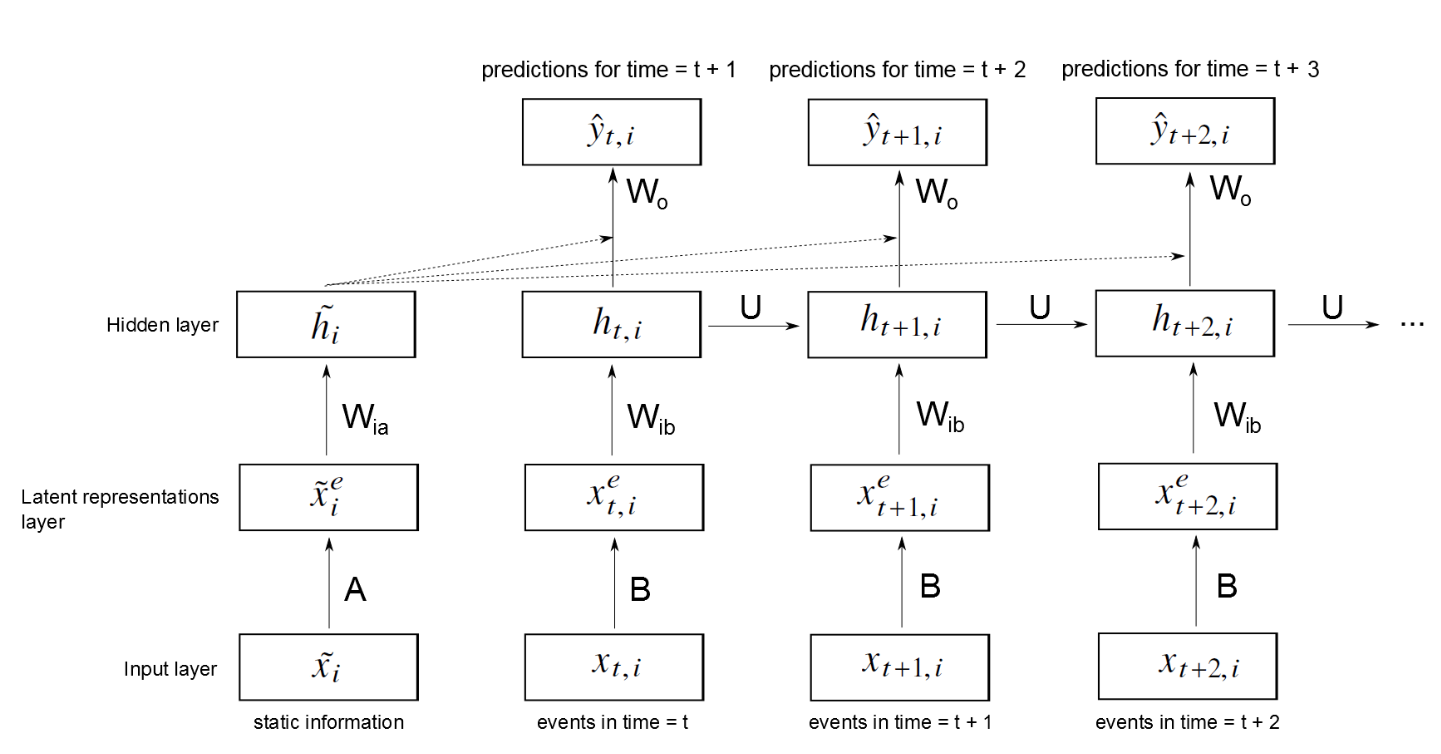
\includegraphics[width=6.5in]{rnnframework.png}
        \caption{RNN framework}
        \medskip
    \end{figure}
    A framework is created in the study conducted by Esteban, et al. wherein static and dynamic data of patients were used as predictors of future clinical events for several RNN implementations. It shows that the static information was first fed into an independent Feedforward Neural Network and the dynamic information into the RNN. Afterward they then concatenated the hidden layers of both networks and provided the information into the output layer.
    
    As shown in the figure, the networks are fed latent representations of the data. The latent representations are computed by applying linear transformation on the raw input, which contains dynamic data and static data of the patient, except for the input for the independent network which only contains the static data of the patient. From the output of the network, a cost is calculated, the cost function applied was based on the Binary Cross Entropy function. [19]
    \FloatBarrier
\chapter{Project Design and Methodology}
\section{Conceptual Framework}
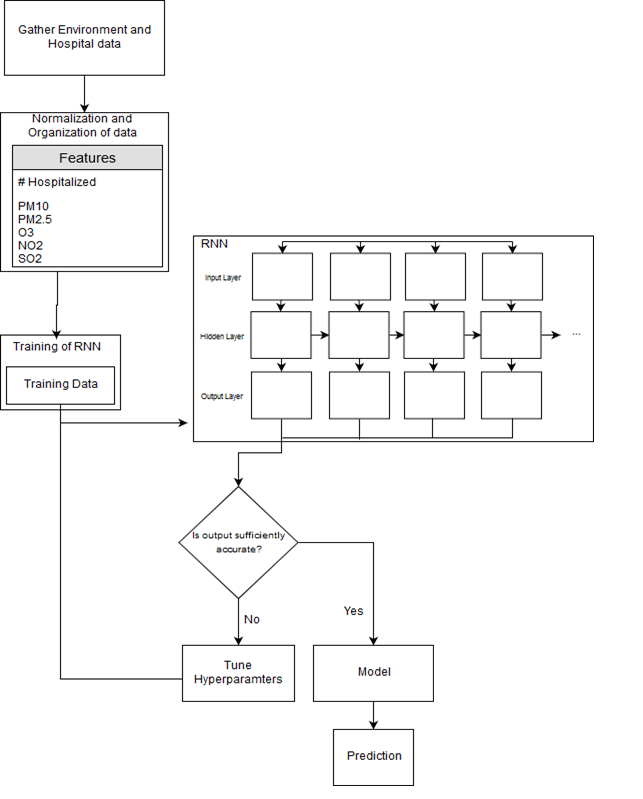
\includegraphics[height=6in]{conframework.png}
\section{Methodology}
    \subsection{Gather environment and hospitalization data}
    The proponents will collate publicly released data from local institutions which contain the variables needed. These variables contain the dates when the data was collected, PM10 concentration, PM2.5 concentrations and number of hospitalized individuals caused by lung diseases. 
    \subsection{Organizing data}
    The proponents will then organize the data into two CSV files, a training set, and a test set.
    \subsection{Defining, Training and Fitting the Model}
    The proponents will then define the number of layers, neurons, and number of features that the LSTM model will have. Then multiple iterations of training will be performed to realize the ideal number of epochs and batch sizes that would be fitted to the model.
    \subsection{Evaluating the Model}
    The proponents will then run the trained model on the test set which would then collect all predictions and calculate an error score. The output shall be the calculated Root Mean Squared Error (RMSE) that gives error in the same units as the variable itself. The data will be presented in a graph format to illustrate the improvement of the model over time.
    \subsection{Implementing the Model}
    Upon achieving an acceptable accuracy, the model will then be implemented by the proponents in a real-world scenario which collects data from several sensors.
\end{document}
